% !TEX root = ../../../main.tex

\toggletrue{image}
\toggletrue{imagehover}
\chapterimage{loop}
\chapterimagetitle{\uppercase{Loop}}
\chapterimageurl{https://xkcd.com/1411/}
\chapterimagehover{Ugh, today's kids are forgetting the old-fashioned art of absentmindedly reading the same half-page of a book over and over and then letting your attention wander and picking up another book.}

\chapter{Schleifen}
\label{chapter-schleifen}

In diesem Kapitel möchten wir ein neues Programmierkonzept kennenlernen, um eine Folge von Befehlen durch Python wiederholt ausführen zu lassen. Mit einer \textbf{Schleife} kann Python die Wiederholung von Befehlen direkt übernehmen, ohne dass wir die Befehle mehrmals eintippen müssen. Es gibt in Python zwei Schleifentypen. Wir kümmern uns zunächst nur um einen Schleifentyp -- die \lstinline{for}-Schleife. Der andere Schleifentyp (\lstinline{while}-Schleife) verschieben wir auf einen späteren Zeitpunkt. Die Lernziele für dieses Kapitel lauten:

\newcommand{\schleifenLernziele}{
\begin{todolist}
\item Sie verwenden eine \lstinline{for}-Schleife, um Befehle wiederholt ausführen zu lassen und somit ein Python-Programm kompakter zu gestalten.
\item Sie notieren den Programmablauf für ein gegebenes Python-Programm, ohne dabei das Programm am Computer ausführen zu lassen.
\end{todolist}
}

\lernziel{\autoref{chapter-schleifen}, \nameref{chapter-schleifen}}{\protect\schleifenLernziele}

\schleifenLernziele

\section{Quadrat ultra kompakt}

Bislang waren die \say{Turtle-Programme} meist sehr repetitiv. Bereits im Programm für das Quadrat mit der Seitenlänge $100$ (\autoref{lst-quadrat}) wiederholt sich der Funktionsaufruf \lstinline{fd(100)} und \lstinline{lt(90)} jeweils viermal. Wir können nun in Python ein Programm erstellen (siehe \autoref{lst-for-loop-quad}), um diese beiden Funktionsaufrufe durch Python viermal wiederholen zu lassen.

\begin{lstlisting}[caption={Zeile vier und fünf wird jeweils viermal ausgeführt (\graybgtexttt{quadrat\_loop.py}).}, label=lst-for-loop-quad]
import turtle

for i in [1, 2, 3, 4]:
    turtle.fd(100)
    turtle.lt(90)
turtle.done()
\end{lstlisting}

Die \lstinline{for}-Schleife besteht aus zwei Teilen (Schleifenkopf und Schleifenkörper):

\begin{itemize}
	\item \textbf{Schleifenkopf}: \lstinline{for} und \lstinline{in} sind Schlüsselwörter von Python und wir müssen diese exakt so notieren. Dazwischen müssen wir eine \textbf{Variable} angeben. Danach notieren wir in den \textbf{eckigen Klammern} so viele Werte, wie Wiederholungen durchgeführt werden sollen. Den Schleifenkopf beenden wir mit einem \textbf{Doppelpunkt}.
\end{itemize}

\begin{example}
	In \autoref{lst-for-loop-quad} befindet sich der Schleifenkopf in Zeile $3$. Die Variable ist \lstinline{i} und es sind vier Werte in den eckigen Klammern notiert. Es werden deshalb vier Wiederholungen durchgeführt.
\end{example}

\begin{itemize}
	\item \textbf{Schleifenkörper}: In diesem Schleifenteil notieren wir die Befehle, welche wiederholt ausgeführt werden sollen. Diese Befehle müssen wir gleichmässig \textbf{einrücken}. Alle eingerückten Befehle müssen denselben Abstand zum \say{Rand} besitzen. Die Einrückung dient \textbf{nicht} zur optischen \say{Verschönerung}. Nur durch die Einrückung (eng. indentation) weiss Python, welche Befehle wiederholt werden müssen. Die eingerückten Befehle bilden den Schleifenkörper.
\end{itemize}

\begin{example}
	In \autoref{lst-for-loop-quad} bilden die Zeilen \num{4} und \num{5} den Schleifenkörper, da diese Zeilen eingerückt sind. Zeile \num{6} gehört nicht mehr dazu, da die Zeile nicht mehr eingerückt ist.
\end{example}

\begin{cleancode}[Leerzeichen 2]
In den eckigen Klammern wird \textbf{nach} einem Komma ein Leerzeichen eingefügt.
\end{cleancode}

\section{Typische Fehlerquellen}

Achten Sie beim Programmieren auf die folgenden, typischen Fehler:

\begin{itemize}
	\item Schlüsselwörter falsch geschrieben.
	\item Doppelpunkt am Ende des Schleifenkopfs vergessen.
	\item Schleifenkörper ist nicht korrekt eingerückt.
\end{itemize}
\autoref{lst-for-loop-quad-errors} zeigt ein fehlerhaftes Programm mit drei Fehlern. In Zeile 3 ist das Schlüsselwort \lstinline{IN} nicht korrekt geschrieben und es fehlt der Doppelpunkt am Ende der Zeile. In Zeile \num{5} ist die Einrückung nicht korrekt. Der Befehl muss um ein Leerzeichen nach links gerückt werden.

\begin{lstlisting}[caption={Fehlerhaftes Programm (\graybgtexttt{quadrat\_loop\_fehler.py}).}, label=lst-for-loop-quad-errors]
import turtle

for k IN [1, 2, 3, 4]
   turtle.fd(100)
    turtle.lt(90)
turtle.done()
\end{lstlisting}

\begin{hinweis}
Die Variable im Schleifenkopf muss nicht \lstinline{i} heissen. Es handelt sich um eine \say{gewöhnliche} Variable. Sie können den Namen selbst wählen.
\end{hinweis}

\section{Aufgaben}

In den folgenden Aufgaben setzen Sie sich mit der \lstinline{for}-Schleife auseinander.

\subsection{Aufgabe 1}

Kürzen Sie das Programm aus \autoref{lst-dreieck-schleife} mit einer \lstinline{for}-Schleife ab. Notieren Sie das Programm direkt hier auf dem Papier.

\begin{minipage}{0.6\textwidth}
\centering
\fillwithgrid{1.9in}
\end{minipage}
\hfill
\begin{minipage}{0.375\textwidth}
\centering
\begin{lstlisting}[caption={Gleichseitiges Dreieck.}, label=lst-dreieck-schleife]
import turtle

turtle.fd(50)
turtle.lt(120)
turtle.fd(50)
turtle.lt(120)
turtle.fd(50)
turtle.lt(120)
turtle.done()
\end{lstlisting}
\end{minipage}

\subsection{Aufgabe 2}

Notieren Sie mithilfe einer \lstinline{for}-Schleife ein Programm, das ein regelmässiges \num{6}-Eck (siehe \autoref{figure-regelmaessiges-sechseck}) zeichnet. Alle Befehle zum Zeichnen müssen im Schleifenkörper notiert werden.

\begin{hinweis}
Ein regelmässiges $n$-Eck ist ein Vieleck mit $n$ gleich langen Seiten, dessen $n$ Innenwinkel alle gleich gross sind.
\end{hinweis}

\begin{figure}[htb]
\centering
\begin{minipage}{0.55\textwidth}
\centering
\fillwithgrid{2in}
\end{minipage}
\hfill
\begin{minipage}{0.375\textwidth}
\centering
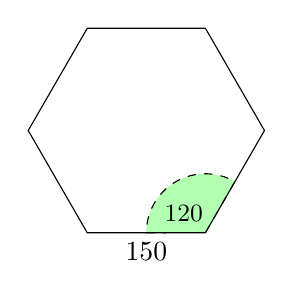
\begin{tikzpicture}
	\draw[fill=green!30, thin, dashed] (1,0) -- ++(60:0.75cm) arc (60:180:0.75cm) -- (0.5,0);
	\draw (1,0) -- ++(60:1.5cm) -- ++(120:1.5cm) -- ++(180:1.5cm) -- ++(240:1.5cm) -- ++(300:1.5cm) to node[below] {\num{150}} ++(360:1.5cm);
	\node at (0.725, 0.25) {\small \qty{120}{\degree}};
\end{tikzpicture}
\caption{Ein regelmässiges \num{6}-Eck mit Seitenlänge \num{150}.}
\label{figure-regelmaessiges-sechseck}
\end{minipage}
\end{figure}

\section{Programmablauf}

Mit dem Programmablauf meinen wir die konkrete Reihenfolge der Befehle, wenn wir ein Programm ausführen. Wir notieren darin die Reihenfolge der Code-Zeilen. Zu jeder Code-Zeile notieren wir auch noch den Speicherinhalt aller selbstdefinierten Variablen.

\begin{example}
Wir schauen uns den Programmablauf aus \autoref{lst-programmablauf-quadrat} in \autoref{table-programmablauf-quadrat} an.

\begin{table}[htb]
\centering
\begin{minipage}{0.4\textwidth}
\centering
\begin{tabular}{cc}
\toprule
\textbf{Code-Zeile} & \textbf{Speicherinhalt der Variablen} \\
			   & Variablenname \\
			   & \lstinline[]$i$ \\
\midrule
1 & $\varnothing$ \\
2 & $\varnothing$ \\ \hline
3 & 1 \\
4 & 1 \\
5 & 1 \\ \hline
3 & 2 \\
4 & 2 \\
5 & 2 \\ \hline
3 & 3 \\
4 & 3 \\
5 & 3 \\ \hline
3 & 4 \\
4 & 4 \\
5 & 4 \\
3 & 4 \\
6 & 4 \\
\bottomrule
\end{tabular}
\caption{Wir notieren den Speicherinhalt immer \textbf{nachdem} die Code-Zeile ausgeführt wurde.}
\label{table-programmablauf-quadrat}
\end{minipage}
\hfill
\begin{minipage}{0.45\textwidth}
\centering
	\begin{lstlisting}[caption={Zeile vier und fünf wird jeweils viermal ausgeführt (\graybgtexttt{quadrat\_loop.py}).}, label={lst-programmablauf-quadrat}]
import turtle

for i in [1, 2, 3, 4]:
    turtle.fd(100)
    turtle.lt(90)
turtle.done()
\end{lstlisting}

\begin{important}
	Der gespeicherte Wert in der Variablen \lstinline{i} wird während des Programmablaufs verändert. Der zuvor gespeicherte Wert in der Variablen \lstinline{i} wird durch den neuen Wert \textbf{ersetzt}. Wir sagen auch, dass der Wert überschrieben wird. Der zuvor gespeicherte Wert ist nicht mehr vorhanden.
\end{important}

\end{minipage}
\end{table}

Durch den Programmablauf aus \autoref{table-programmablauf-quadrat} wird nun auch deutlich, warum ein benannter Speicherplatz als \textbf{Variable} bezeichnet wird. Der Wert im Speicherplatz kann \textbf{variieren}.

\end{example}

\section{Aufgaben}

In den folgenden Aufgaben setzen Sie sich mit Programmablauf auseinander.

\subsection{Aufgabe 1}

Das \autoref{lst-programmablauf-print} ist gegeben. Lesen Sie das Programm zunächst durch. Klären Sie unbekannte Elemente.  Beginnen Sie dann mit den Teilaufgaben.

\begin{lstlisting}[caption={Das Programm erzeugt eine Ausgabe in der Konsole.}, label={lst-programmablauf-print}]
for i in [1, 2, 3, 4, 5, 6, 7, 8, 9, 10]:
    print(<@\color{textcolor}f@>"Der Körper wird zum <@\color{keywordcolor}\{\color{black}i\color{keywordcolor}\}@>. Mal ausgeführt.")
\end{lstlisting}

\begin{enumerate}
\item Notieren Sie die Konsolenausgabe des Programms, wenn man es ausführen würde.

\fillwithgrid{2.5in}

\item Erstellen Sie für das Programm einen Programmablauf wie in \autoref{table-programmablauf-quadrat} gezeigt.

\end{enumerate}

\begin{table}[htb]
\centering
\begin{minipage}{0.45\textwidth}
\begin{tabular}{cc}
\toprule
\textbf{Code-Zeile} & \textbf{Speicherinhalt der Variablen} \\
			   & \lstinline[]$i$ \\
\midrule
& \\ \hline
& \\ \hline
& \\ \hline
& \\ \hline
& \\ \hline
& \\ \hline
& \\ \hline
& \\ \hline
& \\ \hline
& \\ \hline
& \\ \hline
& \\
\bottomrule
\end{tabular}
\end{minipage}
\hfill
\begin{minipage}{0.45\textwidth}
\begin{tabular}{cc}
\toprule
\textbf{Code-Zeile} & \textbf{Speicherinhalt der Variablen} \\
			   & \lstinline[]$i$ \\
\midrule
& \\ \hline
& \\ \hline
& \\ \hline
& \\ \hline
& \\ \hline
& \\ \hline
& \\ \hline
& \\ \hline
& \\ \hline
& \\ \hline
& \\ \hline
& \\
\bottomrule
\end{tabular}
\end{minipage}
\end{table}

\subsection{Aufgabe 2}

Das \autoref{lst-programmablauf-quadratwurzeln} ist gegeben. Lesen Sie das Programm zunächst durch. Klären Sie unbekannte Elemente.  Beginnen Sie dann mit den Teilaufgaben.

\begin{lstlisting}[caption={Das Programm berechnet die Quadratwurzeln der vorgegebenen Zahlen.}, label={lst-programmablauf-quadratwurzeln}]
import math

for k in [49, 64, 100, 16, 36, 4]:
    quadratwurzel = math.sqrt(k)
    print(<@\color{textcolor}f@>"Die Quadratwurzel von <@\color{keywordcolor}\{\color{black}k\color{keywordcolor}\}@> ist <@\color{keywordcolor}\{\color{black}quadratwurzel\color{keywordcolor}\}@>.")
\end{lstlisting}

\begin{enumerate}
\item Notieren Sie die Konsolenausgabe des Programms, wenn man es ausführen würde.

\fillwithgrid{2.5in}

\item Erstellen Sie für das Programm einen Programmablauf wie in \autoref{table-programmablauf-quadrat} gezeigt.

\end{enumerate}

\begin{table}[htb]
\centering
\begin{minipage}{0.45\textwidth}
\begin{tabular}{ccc}
\toprule
\textbf{Code-Zeile} & \multicolumn{2}{c}{\textbf{Speicherinhalt der Variablen}} \\
			   & \lstinline[]$k$ & \lstinline[]$quadratwurzel$ \\
\midrule
1 & $\varnothing$ & $\varnothing$ \\ \hline
2 & $\varnothing$ & $\varnothing$ \\ \hline
& & \\ \hline
& & \\ \hline
& & \\ \hline
& & \\ \hline
& & \\ \hline
& & \\ \hline
& & \\ \hline
& & \\ \hline
& & \\ \hline
& & \\ \hline
& & \\ \hline
& & \\ \hline
& & \\ \hline
& & \\
\bottomrule
\end{tabular}
\end{minipage}
\hfill
\begin{minipage}{0.45\textwidth}
\begin{tabular}{ccc}
\toprule
\textbf{Code-Zeile} & \multicolumn{2}{c}{\textbf{Speicherinhalt der Variablen}} \\
			   & \lstinline[]$k$ & \lstinline[]$quadratwurzel$ \\
\midrule
& & \\ \hline
& & \\ \hline
& & \\ \hline
& & \\ \hline
& & \\ \hline
& & \\ \hline
& & \\ \hline
& & \\ \hline
& & \\ \hline
& & \\ \hline
& & \\ \hline
& & \\ \hline
& & \\ \hline
& & \\ \hline
& & \\ \hline
& & \\
\bottomrule
\end{tabular}
\end{minipage}
\end{table}


\section{Tipparbeit sparen}

\subsection{\lstinline{range}-Funktionsaufruf}

Wir können den Schleifenkopf etwas kompakter gestalten, in dem wir die eckigen Klammern inklusive Inhalt durch einen \lstinline{range}-Funktionsaufruf ersetzen. \autoref{lst-for-loop-quad-range} zeigt den Einsatz der \textbf{eingebauten Funktion}. Wir können uns den Funktionsaufruf so vorstellen, als würden wir in den eckigen Klammern die Zahlen $0$, $1$, $2$ und $3$ notieren (siehe \autoref{lst-for-loop-quad-range-comparison}).

\begin{figure}[htb]
\centering
\begin{minipage}{0.45\textwidth}
\centering
	\begin{lstlisting}[caption={\graybgtexttt{quadrat\_loop\_range.py}}, label={lst-for-loop-quad-range}]
import turtle

for i in range(4):
    turtle.fd(100)
    turtle.lt(90)
turtle.done()
\end{lstlisting}
\end{minipage}
\hfill
\begin{minipage}{0.45\textwidth}
\centering
\begin{lstlisting}[caption={\graybgtexttt{quadrat\_loop.py}}, label={lst-for-loop-quad-range-comparison}]
import turtle

for i in [0, 1, 2, 3]:
    turtle.fd(100)
    turtle.lt(90)
turtle.done()
\end{lstlisting}
\end{minipage}
\end{figure}

\vspace{-0.25cm}

Es gibt verschiedene Möglichkeiten die \lstinline{range}-Funktion aufzurufen. Die \textbf{Reihenfolge} der Argumente ist dabei stets zu beachten.

\begin{itemize}
	\item \lstinline{range(stop)}: erzeugt den Zahlenbereich $0$ bis $\texttt{stop}-1$
	\item \lstinline{range(start, stop)}: erzeugt den Zahlenbereich \lstinline{start} bis $\texttt{stop}-1$
	\item \lstinline{range(start, stop, step)}: wie zuvor, aber mit der Schrittgrösse \lstinline{step}
\end{itemize}

\vspace{-0.25cm}

\begin{important}
Das Argument \lstinline{start} ist in der ersten Variante optional. Standardmässig wird dann für \lstinline{start} die Zahl \num{0} benutzt. In der ersten und zweiten Variante ist das Argument \lstinline{step} nicht vorhanden. Es ist auch optional. Es wird dann standardmässig \num{1} für \lstinline{step} benutzt.
\end{important}

\begin{example}
Konkrete \texttt{range}-Funktionsaufrufe und deren Ergebnisse:
\begin{itemize}
\item \lstinline{range(5)} erzeugt die Zahlen $0$, $1$, $2$, $3$ und $4$.
\item \lstinline{range(3, 6)} erzeugt die Zahlen $3$, $4$ und $5$.
\item \lstinline{range(0, 10, 2)} erzeugt die Zahlen $0$, $2$, $4$, $6$ und $8$.
\end{itemize}

\end{example}

\vspace{-0.25cm}

\subsection{\lstinline{import}-Aliasing}

Unsere Programme werden noch kompakter, wenn wir bei \lstinline{import}-Anweisungen einen Alias (dt. Parallelbezeichnung) verwenden. Dadurch müssen wir nicht jedes Mal den vollständigen Modulnamen verwenden, sondern den von uns gewählten Alias. \autoref{lst-import-alias} zeigt ein Beispiel.

\begin{lstlisting}[caption={Das Turtle-Modul erhält in Zeile $1$ die Bezeichnung \lstinline{t}. Danach können wir die Befehle aus diesem Modul nur noch mit dieser Bezeichnung verwenden (\graybgtexttt{quadrat\_alias.py}).}, label={lst-import-alias}]
import turtle as t

for i in range(4):
    t.fd(100)
    t.lt(90)
t.done()
\end{lstlisting}

Wir können für \textbf{jeden Modulimport} einen Alias benutzen. Dazu erweitern wir die \lstinline{import}-Anweisung und verwenden am Ende das Schlüsselwort \lstinline{as} mit einem gültigen Namen.

\begin{important}
	Zwei \lstinline{import}-Anweisung sollten \textbf{nicht} den gleichen Alias besitzen.
\end{important}

\newpage

\section{Aufgaben}

In den Aufgaben setzen Sie sich mit dem \lstinline{range}-Funktionsaufruf und \lstinline{import}-Aliasing auseinander.

\subsection{Aufgabe 1}

\begin{enumerate}
\item Notieren Sie die Konsolenausgabe für das Programm aus \autoref{lst-range-aufgabe-1}.

\begin{minipage}[c][1in][c]{0.35\textwidth}
\fillwithgrid{0.9in}
\end{minipage}
\hfill
\begin{minipage}[c][1in][c]{0.6\textwidth}
\begin{lstlisting}[caption={Aufgabe 1}, label={lst-range-aufgabe-1}]
for zahl in range(8):
    print(zahl)
\end{lstlisting}
\end{minipage}

\item Notieren Sie die Konsolenausgabe für das Programm aus \autoref{lst-range-aufgabe-2}.

\begin{minipage}[c][1in][c]{0.35\textwidth}
\fillwithgrid{0.9in}
\end{minipage}
\hfill
\begin{minipage}[c][1in][c]{0.6\textwidth}
\begin{lstlisting}[caption={Aufgabe 2}, label={lst-range-aufgabe-2}]
for zahl in range(1, 8):
    print(zahl)
\end{lstlisting}
\end{minipage}

\item Notieren Sie die Konsolenausgabe für das Programm aus \autoref{lst-range-aufgabe-3}.

\begin{minipage}[c][1in][c]{0.35\textwidth}
\fillwithgrid{0.9in}
\end{minipage}
\hfill
\begin{minipage}[c][1in][c]{0.6\textwidth}
\begin{lstlisting}[caption={Aufgabe 3}, label={lst-range-aufgabe-3}]
for zahl in range(8, 1):
    print(zahl)
\end{lstlisting}
\end{minipage}

\item Notieren Sie die Konsolenausgabe für das Programm aus \autoref{lst-range-aufgabe-4}.

\begin{minipage}[c][1in][c]{0.35\textwidth}
\fillwithgrid{0.9in}
\end{minipage}
\hfill
\begin{minipage}[c][1in][c]{0.6\textwidth}
\begin{lstlisting}[caption={Aufgabe 4}, label={lst-range-aufgabe-4}]
for zahl in range(1, 50, 5):
    print(zahl)
\end{lstlisting}
\end{minipage}

\item Notieren Sie die Konsolenausgabe für das Programm aus \autoref{lst-range-aufgabe-5}.

\begin{minipage}[c][1in][c]{0.35\textwidth}
\fillwithgrid{0.9in}
\end{minipage}
\hfill
\begin{minipage}[c][0.75in][c]{0.6\textwidth}
\begin{lstlisting}[caption={Aufgabe 5}, label={lst-range-aufgabe-5}]
for zahl in range(50, -20, -10):
    print(zahl)
\end{lstlisting}
\end{minipage}

\item Notieren Sie die Konsolenausgabe für das Programm aus \autoref{lst-range-aufgabe-6}.

\begin{minipage}[c][1in][c]{0.35\textwidth}
\fillwithgrid{0.9in}
\end{minipage}
\hfill
\begin{minipage}[c][0.75in][c]{0.6\textwidth}
\begin{lstlisting}[caption={Aufgabe 5}, label={lst-range-aufgabe-6}]
for zahl in range(1900, 2051, 25):
    print(zahl)
\end{lstlisting}
\end{minipage}

\end{enumerate}

\subsection{Aufgabe 2}

Passen Sie das Programm aus \autoref{lst-range-print} so an, dass im Schleifenkopf ein passender \lstinline{range}-Funktionsaufruf stattfindet. Sie können die Korrektur direkt im Listing vornehmen.

\vspace{0.5cm}

\begin{lstlisting}[caption={Ersetzen Sie den Schleifenkopf.}, label={lst-range-print}]
for i in [1, 2, 3, 4, 5, 6, 7, 8, 9, 10]:
    print(<@\color{textcolor}f@>"Der Körper wird zum <@\color{keywordcolor}\{\color{black}i\color{keywordcolor}\}@>. Mal ausgeführt.")
\end{lstlisting}

\subsection{Aufgabe 3}

Schreiben Sie das Programm aus \autoref{lst-range-alias-turtle} so um, dass ein \lstinline{import}-Alias, ein passender \lstinline{range}-Funktionsaufruf und eine passende Variable für die Seitenlänge benutzt wird.

\begin{figure}[htb]
\begin{minipage}{0.45\textwidth}
\fillwithgrid{2in}
\end{minipage}
\hfill
\begin{minipage}{0.5\textwidth}
\begin{lstlisting}[caption={Es wird ein regelmässiges \num{6}-Eck mit der Seitenlänge 150 gezeichnet.}, label={lst-range-alias-turtle}]
import turtle

for i in [1, 2, 3, 4, 5, 6]:
    turtle.fd(150)
    turtle.lt(60)
turtle.done()
\end{lstlisting}
\end{minipage}
\end{figure}

\subsection{Aufgabe 4}

Es ist das Programm aus \autoref{lst-range-alias-math-random} gegeben. Studieren Sie das Programm. Klären Sie unbekannte Programmierelemente. Lösen Sie dann die folgende Aufgabe: Schreiben Sie das Programm so um, dass ein \lstinline{import}-Alias und ein passender \lstinline{range}-Funktionsaufruf. Schaffen Sie es auch, dass der \lstinline{range}-Funktionsaufruf eine sinnvolle Variable benutzt?

\begin{lstlisting}[caption={Es werden Quadratwurzeln berechnet.}, label={lst-range-alias-math-random}]
import random
import math

for i in [1, 1, 1, 1, 1, 1, 1, 1, 1, 1]:
    zahl = random.randrange(1, 100)
    quadratwurzel = math.sqrt(zahl)
    print(<@\color{textcolor}f@>"Die Quadratwurzel von <@\color{keywordcolor}\{\color{black}zahl\color{keywordcolor}\}@> ist <@\color{keywordcolor}\{\color{black}quadratwurzel\color{keywordcolor}\}@>.")
\end{lstlisting}

\fillwithgrid{\stretch{1}}